\documentclass[10pt]{scrreprt}
\usepackage[utf8]{inputenc}
\usepackage{amsfonts}
\usepackage{amsmath}
\usepackage{amssymb}
\usepackage{commath}
\usepackage[ngerman]{babel}
\usepackage{enumitem}
\usepackage{booktabs}
\usepackage{longtable}
\usepackage{relsize}
\usepackage{pgfplots}
\usepackage{csvsimple}
\usepackage{pgfplotstable}
\usepackage{siunitx}
\usepackage{fancyhdr}
\usepackage{color}
\usepackage{float}
\usepackage{listings}

\definecolor{mygreen}{RGB}{28,172,0} % color values Red, Green, Blue
\definecolor{mylilas}{RGB}{170,55,241}


\lstset{language=Matlab,%
    %basicstyle=\color{red},
    breaklines=true,%
    morekeywords={matlab2tikz},
    keywordstyle=\color{blue},%
    morekeywords=[2]{1}, keywordstyle=[2]{\color{black}},
    identifierstyle=\color{black},%
    stringstyle=\color{mylilas},
    commentstyle=\color{mygreen},%
    showstringspaces=false,%without this there will be a symbol in the places where there is a space
    %numbers=left,%
    %numberstyle={\tiny \color{black}},% size of the numbers
    %numbersep=9pt, % this defines how far the numbers are from the text
    emph=[1]{for,end,break},emphstyle=[1]\color{red}, %some words to emphasise
    %emph=[2]{word1,word2}, emphstyle=[2]{style},
}

\setlength\parindent{0pt}

\setcounter{chapter}{5}
\setcounter{secnumdepth}{3}
\setcounter{figure}{12}


\pagestyle{fancy}
\fancyhf{}
\lhead{GPET Versuch 5}
\rhead{Tim Luchterhand, Paul Nykiel}
\cfoot{\thepage}

\author{Tim Luchterhand, Paul Nykiel \protect\\ tim.luchterhand@uni-ulm.de, paul.nykiel@uni-ulm.de}
\title{GPET Versuch 5 --- Hochspannung mit Stanley und Tesla}
\subtitle{Gruppe: Dienstag14}

\begin{document}
        \maketitle
        \section{Spannungsübersetzung beim unbelasteten Transformator}
        \paragraph{Aufgabe}
        In diesem ersten Versuchsteil sollen verschiedene Übersetzungsverhältnisse des
        unbelasteten Transformators betrachtet werden. Bauen Sie dazu die Schaltung mit $R_V = 100\si{\ohm}$
        nach Abbildung~\ref{fig:abb8} auf. Erzeugen Sie ein Sinuseingangssignal $U_{Ein}$ mit Hilfe des Signalgenerators
        des Oszilloskops, $f = 500\si{\hertz}$, $U = 1\si{\volt}_{pp}$.

        \vspace{0.5cm}

        Messen Sie jeweils für die verschiedenen Windungsverhältnisse gemäß Tabelle \ref{tab:mess1} die
        Primärspannung $U_1$, die Sekundärspannung $U_2$ mit den beiden Kanälen des Oszilloskops und
        berechnen Sie das Verhältnis $\frac{U_2}{U_1}$. Übernehmen Sie Tabelle~\ref{tab:mess1} in Ihr Protokoll und ergänzen
        Sie die zu ermittelnden Größen. Diskutieren Sie Ihre Ergebnisse.

        \begin{center}
            \begin{figure}[H]
                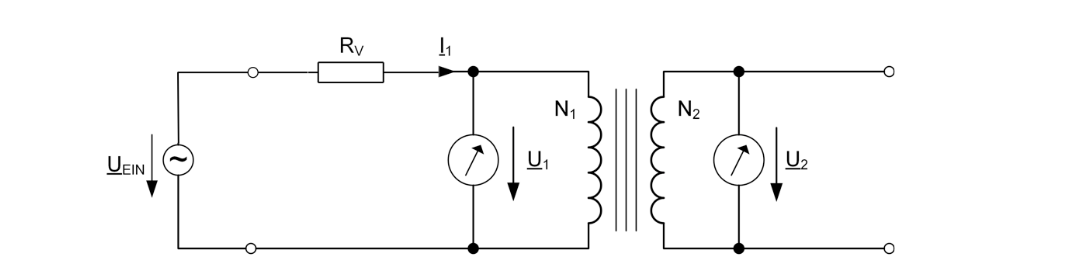
\includegraphics[width=\textwidth]{aufgabenBilder/abbildung8.png}
                \caption{Versuchsaufbau des ersten Teilversuchs: unbelasteter Transformator}
                \label{fig:abb8}
            \end{figure}
        \end{center}

        \paragraph{Protokoll}
        $ $
        \begin{table}[h!]
            \begin{center}
                \pgfplotstabletypeset[
                multicolumn names, % allows to have multicolumn names
                col sep=space, % the seperator in our .csv file
                %string replace*={inf}{$\infty$},
                %string type,
                header=false,
                display columns/0/.style={
                column name=$N_1$, % name of first column
                column type={S},string type},  % use siunitx for formatting
                display columns/1/.style={
                column name=$N_2$,
                column type={S},string type},
                display columns/2/.style={
                column name=$U_1$,
                column type={S},string type},
                display columns/3/.style={
                column name=$U_2$,
                column type={S},string type},
                display columns/4/.style={
                column name=$\dfrac{U_2}{U_1}$,
                column type={S},string type},
                every head row/.style={
                before row={\toprule}, % have a rule at top
                after row={
                 & & $\si{m\volt}_{pp}$ & $\si{m\volt}_{pp}$\\
                \midrule} % rule under units
                },
                every last row/.style={after row=\bottomrule},
                ]{mess1.csv}
                \caption{Messtabelle zu Versuch 5.1}
                \label{tab:mess1}
            \end{center}
        \end{table}

        Wir erwarten folgendes Verhalten:
        \begin{equation*}
            \frac{U_2}{U_1} = \frac{N_2}{N_1}
        \end{equation*}
        In der Realität zeichnet sich jedoch folgendes Verhalten ab
        \begin{eqnarray*}
            \frac{U_2}{U_1} < \frac{N_2}{N_1}\\
            \frac{4}{3} \cdot \frac{U_2}{U_1} \approx \frac{N_2}{N_1}\\
            \Rightarrow \frac{U_2}{U_1} \sim \frac{N_2}{N_1}
        \end{eqnarray*}

        Wie erwartet sind die beiden Verhältnisse zueinander proportional, jedoch
        nicht mit einem Proportionalitätsfaktor von $1$, sondern von ca.~$\frac{4}{3}$.
        Dies lässt sich durch die Unidealität des Transformators erklären, da durch
        Streufelder und den Ohmschen Widerstand der Spule Verluste entstehen.

        %TODO Diskutieren sie ihr Ergebniss
        % U_2/U_1 sollte gleich N_2 / N_1 sein
        % 60mVpp Fehler

        \section{Der belastete Transformator}
        \paragraph{Aufgabe}
        In diesem Versuchteil soll der Einfluss verschiedener Lastwiderstände auf die
        Spannungstransformation bei zwei unterschiedlichen Windungsverhältnissen untersucht werden.
        Bauen Sie dazu die Schaltung mit $R_V = 100\si{\ohm}$ nach Abbildung~\ref{fig:abb9} auf. Als Last $R_L$ verwenden Sie ein
        Potentiometer ($0\ldots1000\si{\ohm}$) dem Sie zusätzlich einen $100\si{\ohm}$ Widerstand in Reihe schalten.
        Als Eingangssignal $U_{Ein}$ stellen Sie am Signalgenerator des Oszilloskops ein Sinussignal
        der Spannung $1 \si{\volt}_{pp}$ und der Frequenz $f = 500\si{\hertz}$ ein.

        \vspace{0.5cm}

        Messen Sie für die Windungsverhältnisse $N_1 : N_2 = 500 : 500$ und $N_1 : N_2 = 250 : 500$
        die Primärspannung $U_1$ sowie die Sekundärspannung $U_2$ für verschiedene Lastwiderstände
        ($100\ldots1000\si{\ohm}$) gemäß Tabelle~\ref{tab:mess2} und berechnen Sie zudem das Verhältnis $\frac{U_2}{U_1}$.
        Übernehmen Sie Tabelle~\ref{tab:mess2} in ihr Protokoll und ergänzen Sie die zu ermittelnden Größen.

        \begin{center}
            \begin{figure}[H]
                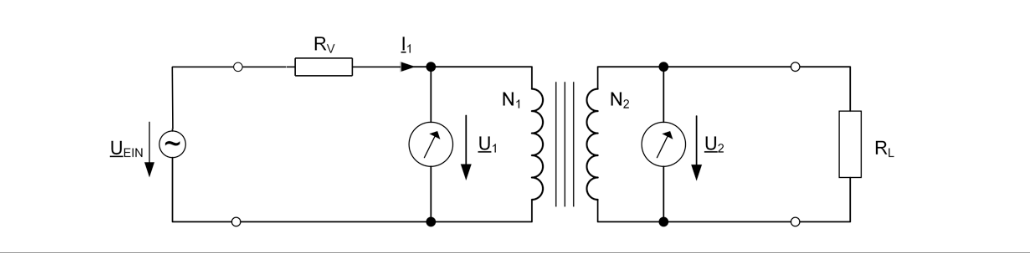
\includegraphics[width=\textwidth]{aufgabenBilder/abbildung9.png}
                \caption{Versuchsaufbau des zweiten Teilversuchs: belasteter Transformator}
                \label{fig:abb9}
            \end{figure}
        \end{center}

        Tragen Sie für die beiden Windungsverhältnisse $N_1 : N_2 = 500 : 500$ und $N_1 : N_2 = 250 : 500$
        das Spannungsübersetzungsverhältnis $U_2 / U_1$ über den Lastwiderstand $R_L$ auf und
        diskutieren Sie ihre Ergebnisse.

        \paragraph{Protokoll}
        $ $
        \begin{table}[H]
            \begin{center}
                \pgfplotstabletypeset[
                multicolumn names, % allows to have multicolumn names
                col sep=space, % the seperator in our .csv file
                %string replace*={inf}{$\infty$},
                %string type,
                header=false,
                display columns/0/.style={
                column name=$R_L$, % name of first column
                column type={S},string type},  % use siunitx for formatting
                display columns/1/.style={
                column name=$U_1$,
                column type={S},string type},
                display columns/2/.style={
                column name=$U_2$,
                column type={S},string type},
                display columns/3/.style={
                column name=$U_2 / U_1$,
                column type={S},string type},
                display columns/4/.style={
                column name=$U_1$,
                column type={S},string type},
                display columns/5/.style={
                column name=$U_2$,
                column type={S},string type},
                display columns/6/.style={
                column name=$U_2 / U_1$,
                column type={S},string type},
                every head row/.style={
                before row={\toprule \\ & \multicolumn{3}{c}{$500:500$} & \multicolumn{3}{c}{$250:500$}\\}, % have a rule at top
                after row={
                $\si{\ohm}$ & $\si{m\volt}_{pp}$ & $\si{m\volt}_{pp}$ & & $\si{m\volt}_{pp}$ & $\si{m\volt}_{pp}$\\
                \midrule} % rule under units
                },
                every last row/.style={after row=\bottomrule},
                ]{mess2.csv}
                \caption{Messtabelle zu Versuch 5.2}
                \label{tab:mess2}
            \end{center}
        \end{table}
        Windungsverhältnisse 500:500 in \textcolor{green}{grün}, 250:500 in \textcolor{blue}{blau}.
        \begin{center}
            \begin{tikzpicture}
        		\begin{axis}[ymin=0, xmin=0, xlabel = {$R_L$[$\Omega$]}, ylabel = {$U_2/U_1$}]
        			\addplot[color=green] table[x index = {0},
                            y index = {3}] {mess2.csv};
                    \addplot[color=blue] table[x index = {0},
                            y index = {6}] {mess2.csv};
        		\end{axis}
        	\end{tikzpicture}
        \end{center}

        Der Messpunkt der grünen Kurve bei einem Widerstand von $400\si{\ohm}$
        fällt klar aus der Messreihe heraus. Wir gehen von einem Messfehler aus.

        \vspace{0.5cm}

        Eigentlich würde man erwarten, dass beide Kurven konstant bleiben, da
        das Übertragungsverhältnis $\dfrac{N_2}{N_1} = \dfrac{U_2}{U_1}$ sich
        nicht ändern sollte, die Windungszahlen bleiben ja schließlich gleich.
        Beachtet man aber die Verluste, die bei einem nichtidealen
        Transformator auftreten, lässt sich das Verhalten folgendermaßen erklären.
        Ein Stromfluss im Sekundärkreis verursacht Energieverluste durch Streufelder,
        den Ohmschen Widerstand und die Gegeninduktivität M. Bei einem niedrigen
        Stromfluss sind diese Verluste entsprechend niedriger. Da ein hoher Lastwiderstand
        den Stromfluss beschränkt, verhält sich der Transformator mit zunehmendem
        Lastwiderstand immer idealer. Für den Extremfall $R_L \rightarrow \infty$
        verhält sich das System wie in Aufgabe 5.1.

        %TODO Ergebnisse Diskutieren
        %hier so voll rüber transormiert und dan spannungsteiler und so
        %30mVpp Offset

        \section{Kopplungsgrad}
        \paragraph{Aufgabe}
        In diesem Versuchsteil soll der Kopplungsgrad k des Transformators ($N_1 : N_2 = 500 : 500$)
        bei den Frequenzen $f_1 = 500\si{\hertz}$ und $f_2 = 5000\si{\hertz}$ mit Hilfe der in Abschnitt 4.1
        bestimmten Ausdrücke für $L_1$, $L_2$ und $M$ bestimmt werden. (Falls Sie diese Vorbereitungsaufgabe
        nicht lösen konnten, sprechen Sie mit Ihrem Tutor). Zur Berechnung von $L_1$ und $M$
        verwenden Sie den Aufbau nach~\ref{fig:abb10} um die Größen $U_1$ und $I_1$ zu ermitteln. Als
        Eingangssignal erzeugen Sie wieder einen Sinus mit $U = 1\si{\volt}_{pp}$ mit Hilfe des
        Signalgenerators des Oszilloskops. ($R_V = 100\si{\ohm}$)

        \begin{center}
            \begin{figure}[H]
                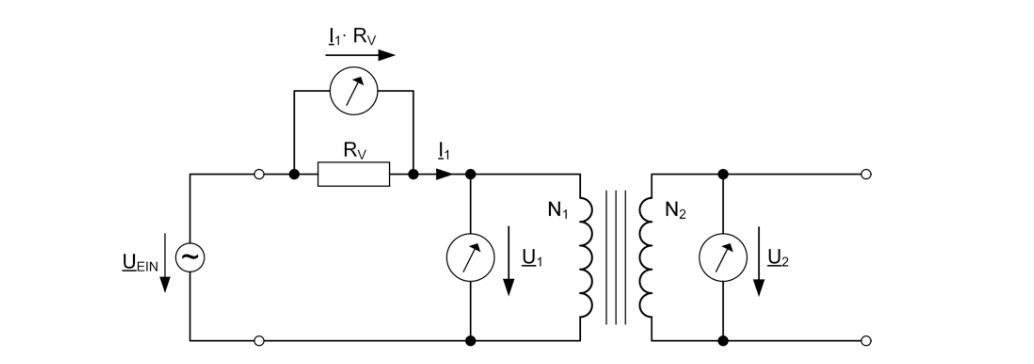
\includegraphics[width=\textwidth]{aufgabenBilder/abbildung10.png}
                \caption{Aufbau zur Ermittlung des Kopplungsgrades}
                \label{fig:abb10}
            \end{figure}
        \end{center}

        Für die Berechnung von $L_2$ muss der Primärstrom $I_1$, sowie der Kurzschlussstrom $I_2$
        ermittelt werden. Bauen Sie hierzu die Schaltung nach~\ref{fig:abb11} auf. Geben Sie hier
        einen Sinus der Spannung $U = 2\si{\volt}_{pp}$ auf die Schaltung und messen Sie die beiden Ströme
        $I_1$ und $I_2$ mit Hilfe der schwarzen VOLTCRAFT-Multimeter (Messbereich mA, Wech-
        selstrom) für die beiden Frequenzen $f_1$ und $f_2$. Beachten Sie, dass das Multimeter beim
        Messen von Wechselgrößen den Effektivwert liefert!

        \begin{center}
            \begin{figure}[H]
                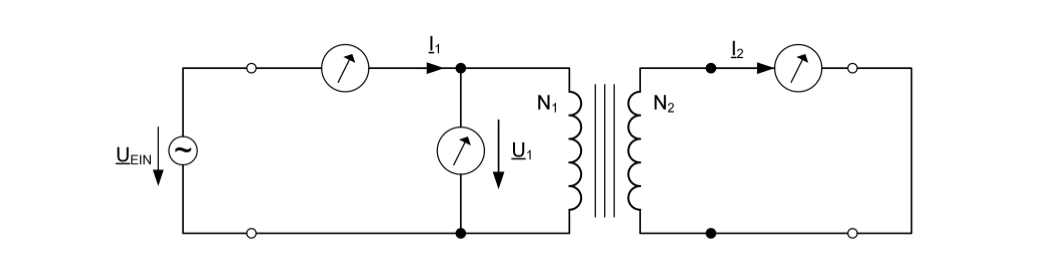
\includegraphics[width=\textwidth]{aufgabenBilder/abbildung11.png}
                \caption{Versuchsaufbau für die Kurzschlussmessungen zur Bestimmung des Kopplungsgrades}
                \label{fig:abb11}
            \end{figure}
        \end{center}

        Nachdem Sie die Größen $L_1$, $L_2$ und $M$ ermittelt haben, berechnen Sie den Kopplungsgrad
        $k$ für die Frequenzen $f_1$ und $f_2$ und diskutieren Sie Ihre Ergebnisse.

        \paragraph{Protokoll}
        %N_2 = N_1 = 500

        % für f = 500Hz
        % Offen:
        % U_1 = 306mV_rms
        % U_2 = 234mV_rms
        % I_1 = 0.917mA
        % Kurzschluss:
        % U_1 = 298mVrms / 301 / 299
        % I_1 = 1.37mArms / 2.04 / 1.98
        % I_2 = 0.38mArms/ 1.52 / 1.45

        % für f = 5kHz
        % Offen:
        % U_1 = 344mVrms
        % U_2 = 251mVrms
        % I_1 = 0.136mArms
        % Kurzschluss:
        % U_1 = 342Vrms
        % I_1 = 0.199mArms
        % I_2 = 0.132mArms

        \begin{equation*}
            N_2 = N_1 = 500
        \end{equation*}

        Für $f=500\si{\hertz}$:
        \begin{eqnarray*}
            U_1 &=& 306\si{m\volt}_{RMS}\\
            U_2 &=& 234\si{m\volt}_{RMS}\\
            {I_1}_{offen} &=& 0.917 \si{m\ampere}_{RMS}\\
            \omega &=& 2 \pi f = 3142 \si{\hertz}\\
            L_1 &=& \dfrac{U_1}{\omega {I_1}_{offen}} = 0.106 \si{\henry}\\
            M &=& L_1 \dfrac{N_2}{N_1} = L_1 = 0.106 \si{\henry}\\
            {I_1}_{k} &=& 2.01\si{m\ampere}_{RMS}\\
            {I_2}_{k} &=& 1.49\si{m\ampere}_{RMS}\\
            L_2 &=& M \cdot \dfrac{{I_1}_{k}}{{I_2}_{k}} =
            0.110 \si{\henry}\\
            k &=& \dfrac{M}{\sqrt{L_1 L_2}} = 0.98
        \end{eqnarray*}

        Für $f=5000\si{\hertz}$:
        \begin{eqnarray*}
            U_1 &=& 344\si{m\volt}_{RMS}\\
            U_2 &=& 251\si{m\volt}_{RMS}\\
            {I_1}_{offen} &=& 0.136 \si{m\ampere}_{RMS}\\
            \omega &=& 2 \pi f = 31416 \si{\hertz}\\
            L_1 &=& \dfrac{U_1}{\omega {I_1}_{offen}} =  0.0805\si{\henry}\\
            M &=& L_1 \frac{N_2}{N_1} = L_1 =  0.0805\si{m\henry}\\
            {I_1}_{k} &=& 0.199\si{m\ampere}_{RMS}\\
            {I_2}_{k} &=& 0.132\si{m\ampere}_{RMS}\\
            L_2 &=& M \cdot \dfrac{{I_1}_{k}}{{I_2}_{k}} =0.121
             \si{\henry}\\
            k &=& \dfrac{M}{\sqrt{L_1 L_2}} = 0.814
        \end{eqnarray*}

        Es fällt auf, dass bei höherer Frequenz der Kopplungsgrad des Transformators
        sinkt. Das bedeutet, dass das System insgesammt schlechter überträgt, ein
        ideales System hätte einen Kopplungsgrad von $1$.

        \textbf{Erklärung:}
        Die Streuinduktivitäten eines nichtidealen Transformators speichern bei höherer
        Frequenz mehr Energie in ihren Magnetfeldern. Es geht also mehr Energie in diesen
        Streufeldern verloren, was dazu führt, dass der Kopplungsgrad abnimmt.


        \section{Frequenzabhängiges Übertragungsverhalten und Phasenschiebung unter Last}
        \paragraph{Aufgabe}
        \begin{center}
            \begin{figure}[H]
                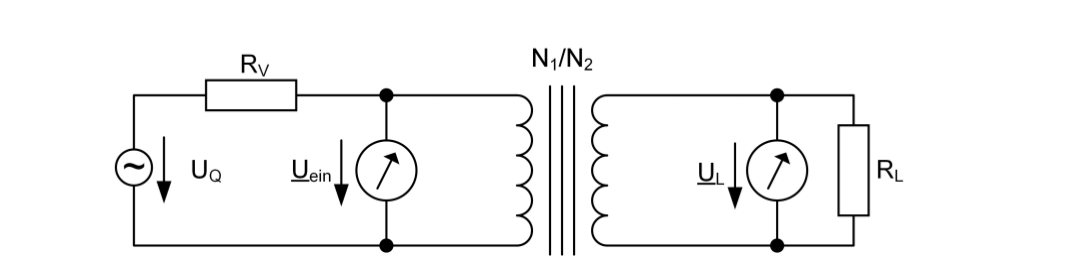
\includegraphics[width=\textwidth]{aufgabenBilder/abbildung12.png}
                \caption{Versuchsaufbau zur Messung des Übertragungsverhalten bei verschiedenen Frequenzen.}
                \label{fig:abb12}
            \end{figure}
        \end{center}

        In diesem letzten Aufgabenteil soll das frequenz- und lastabhängige Übertragungsverhalten
        des Transformators untersucht werden.

        \vspace{0.5cm}

        Messen Sie hierzu mit dem in~\ref{fig:abb12} gezeigten Versuchsaufbau (Transformator mit
        $N_1 = N_2 = 500$ Windungen) die Spannungen $U$ ein und $U_L$ mit Hilfe der beiden Eingangskanäle
        des Oszilloskops als Funktion der Frequenz für die drei Lastwiderstandswerte
        $R_L = \{100\si{\ohm}, 680 \si{\ohm}, 1 \si{k\ohm}\}$. Verwenden Sie hierfür die Sweep-Funktion der MATLAB GUI.
        Setzen Sie die Quellenspannung $U_Q$ mit Hilfe der MATLAB GUI auf $1\si{\volt}$ (Z LOAD = high-Z).
        Nehmen Sie den Betrag und die Phase des Frequenzgangs der Übertragungsfunktion
        $U_2 /U_1 (\omega)$ für Frequenzen zwischen $100\si{\hertz}$ und $100\si{k\hertz}$ (logarithmisch verteilt mit 100
        Frequenzpunkten) für die drei oben genannten Lastwiderstandswerte auf (Hinweis:
        Ermitteln Sie zunächst den Amplitudengang mit der Funktion \glqq{}Sweep --- Frequency\grqq{} und
        anschließend den Phasengang mit der Funktion \glqq{}Sweep --- Phase\grqq{}. Verwenden Sie bei der
        Ermittlung des Phasengangs zur Verbesserung der Qualität der Phasenmessung 4 Mittelungen).

        \vspace{0.5cm}

        Tragen Sie Betrag und Phase von $U_2 /U_1 (\omega)$ für die drei Lastwiderstandswerte in
        einem Bode-Diagramm auf. Diskutieren Sie Ihre Messwerte mit Hilfe Ihrer Ergebnisse aus
        Abschnitt 4.2.

        \paragraph{Protokoll}
        %TODO Betrag und Phase in Bode Diagramm; Messwerte diskutieren
        Die in 4.2 errechente Übertragungsfunktion

        \begin{equation*}
            H = \frac{\underline{U_2}}{\underline{U_1}} = \frac{R_L \cdot N_2 \cdot
            L_{h_1}}{(j \omega L_{S_1} + R_L) \cdot N_1 (L_{H_1} + L_{S_1})}
        \end{equation*}

        \vspace{0.2cm}

        verhält sich für Extremwerte folgendermaßen:

        \begin{eqnarray*}
            H(\omega) &\rightarrow& 0 \ (\omega \rightarrow \infty)\\
            \Rightarrow \frac{\abs{H}}{\text{dB}} &\rightarrow& -\infty \ (\omega \rightarrow \infty)
        \end{eqnarray*}

        Dieses Verhalten lässt sich auch in den folgenden Diagrammen erkennen:
        Für große Frequenzen nimmt die Übertragungsfunktion im logarithmischen
        Diagramm linear ab und geht im Grenzwert $\omega \rightarrow \infty$
        gegen $-\infty$.

        \begin{center}
            \begin{figure}[H]
                \centering
                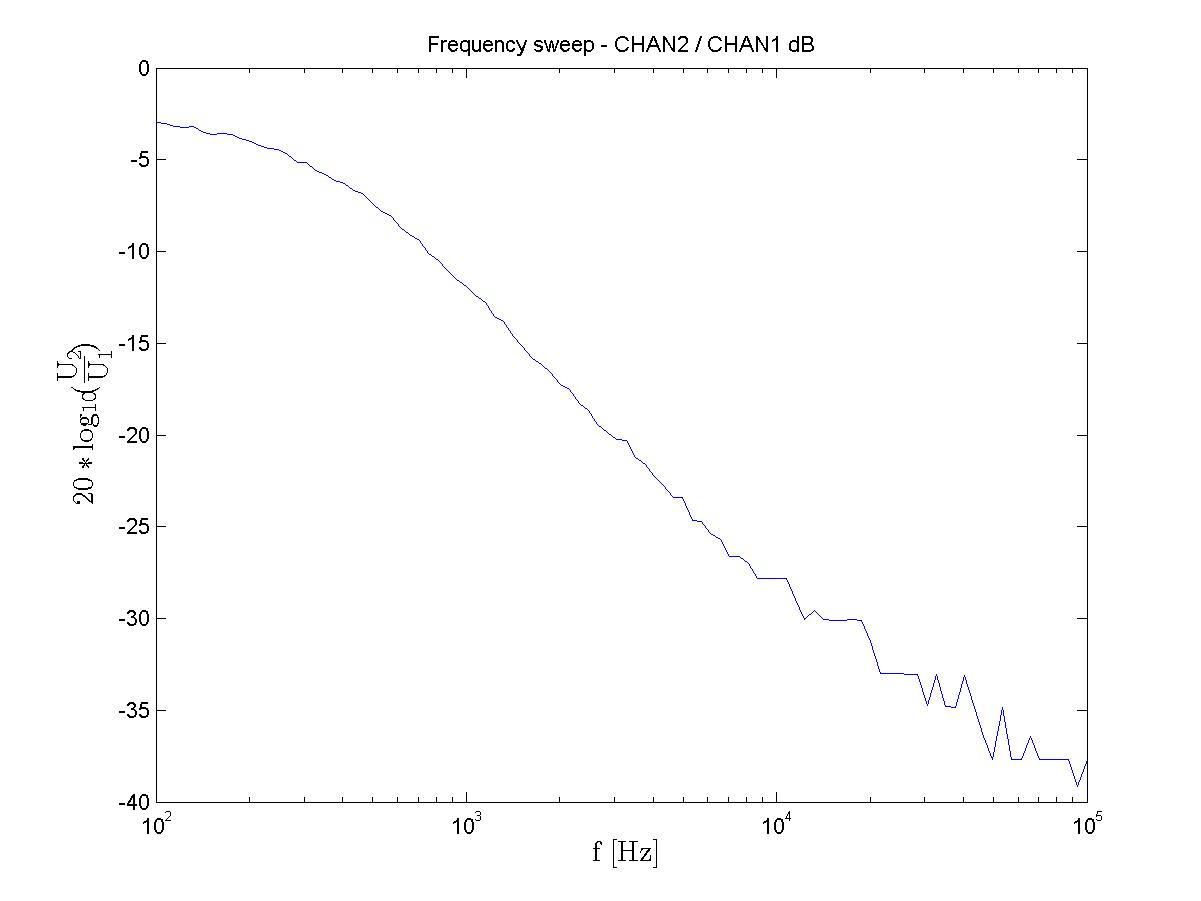
\includegraphics[width=0.9\textwidth]{SchweepVpp_100Ohm_frequencysweep_ylogxlog.jpg}
                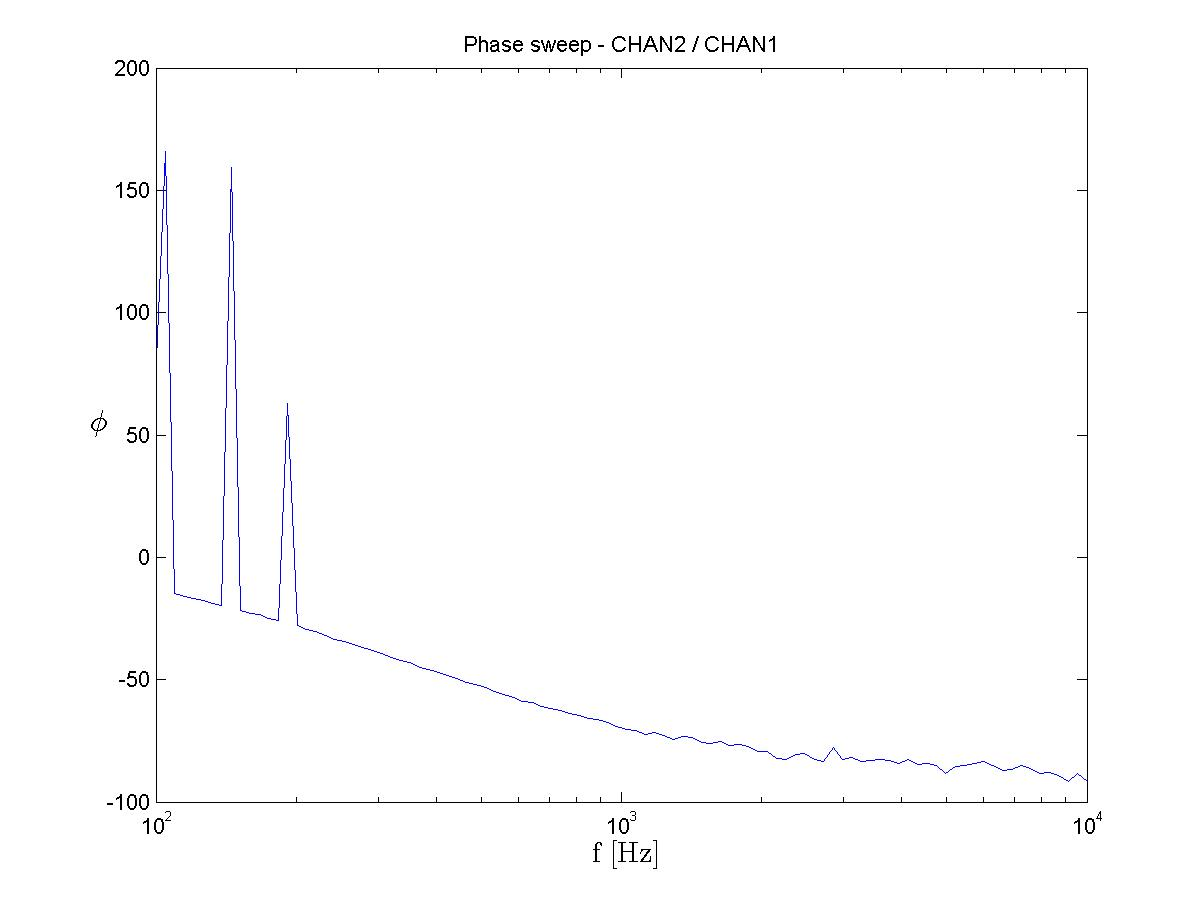
\includegraphics[width=0.9\textwidth]{100OhmKraids_phasesweep_xlog.jpg}
                \caption{Bode-Diagramm mit $R_L = 100\si{\ohm}$}
            \end{figure}

            \begin{figure}[H]
                \centering
                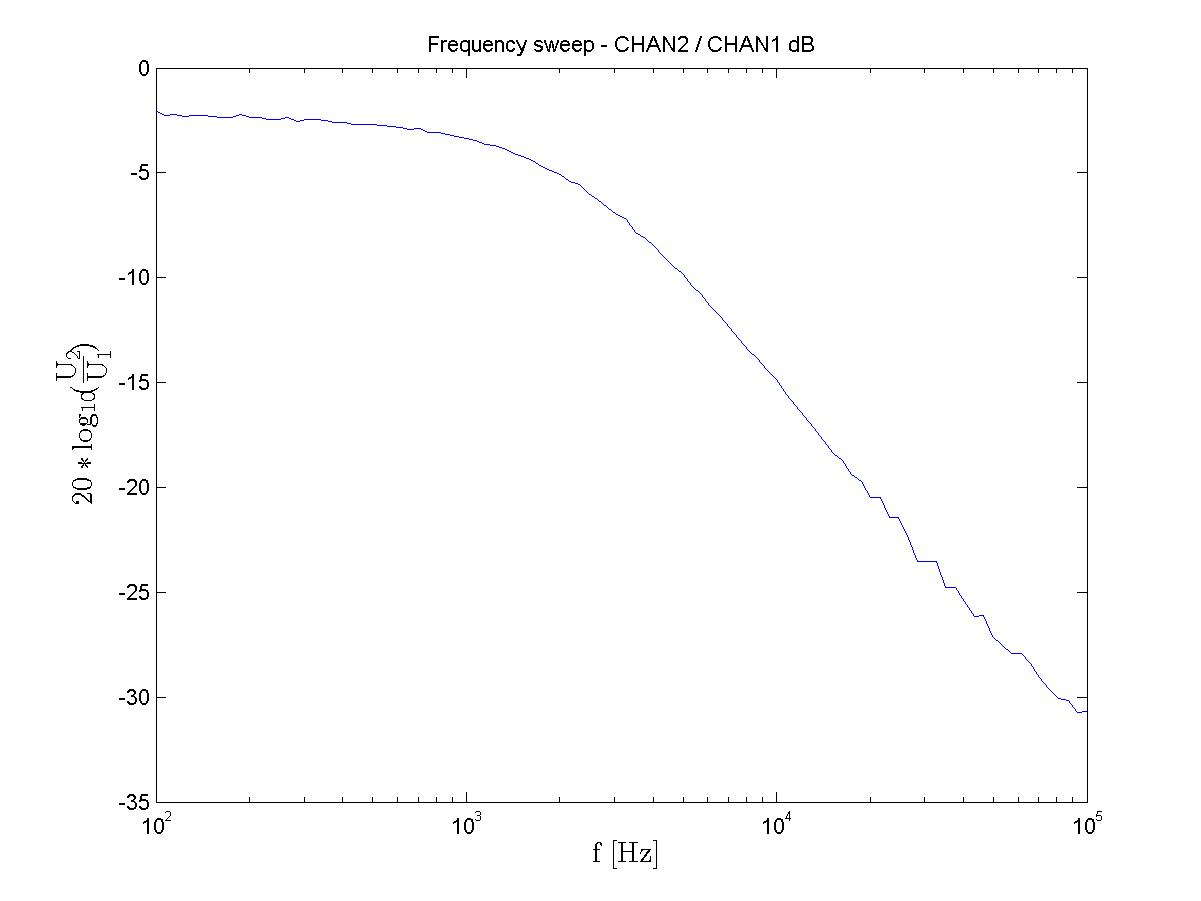
\includegraphics[width=0.9\textwidth]{SchweepVpp_680Ohm_frequencysweep_ylogxlog.jpg}
                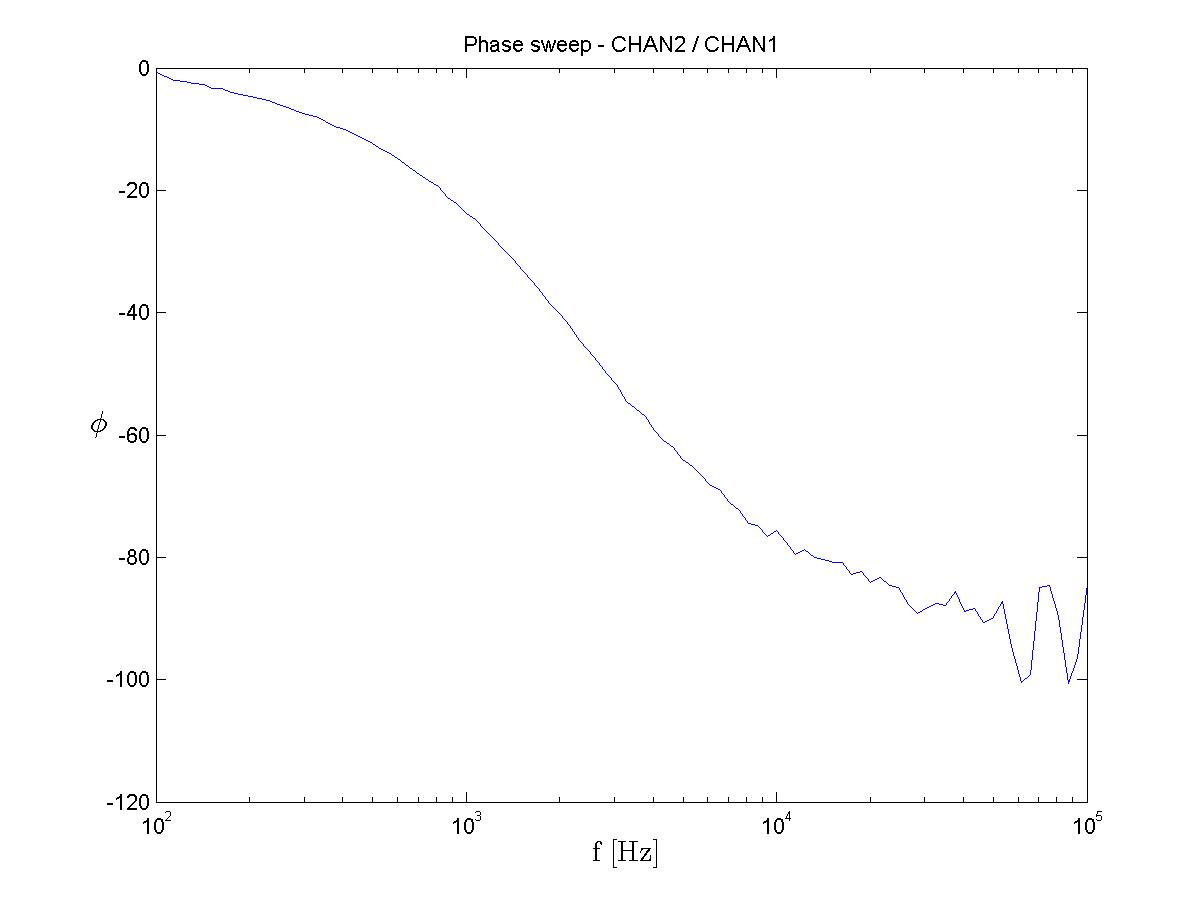
\includegraphics[width=0.9\textwidth]{680OhmNett_phasesweep_xlog.jpg}
                \caption{Bode-Diagramm mit $R_L = 680\si{\ohm}$}
            \end{figure}

            \begin{figure}[H]
                \centering
                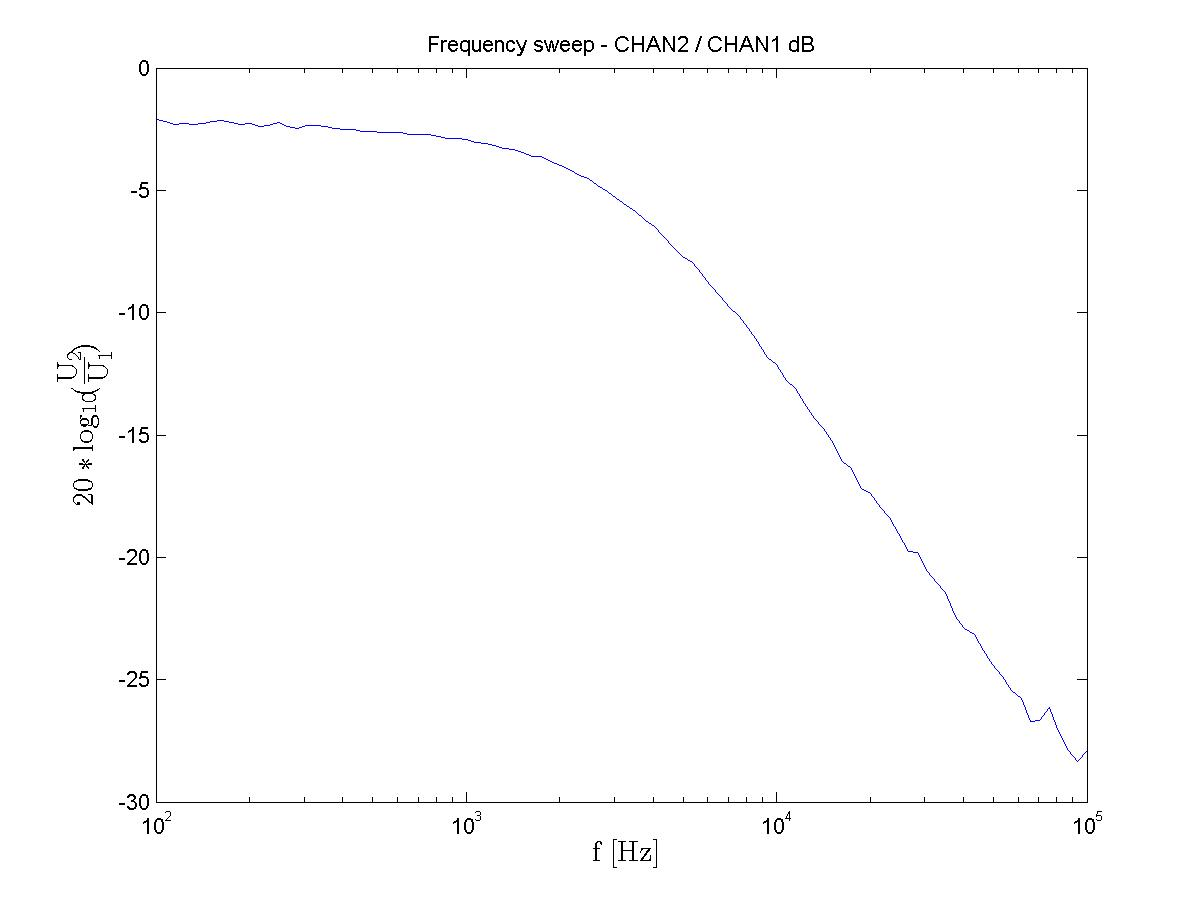
\includegraphics[width=0.9\textwidth]{SchweepeeSchweepVpp_1000Ohm_frequencysweep_ylogxlog.jpg}
                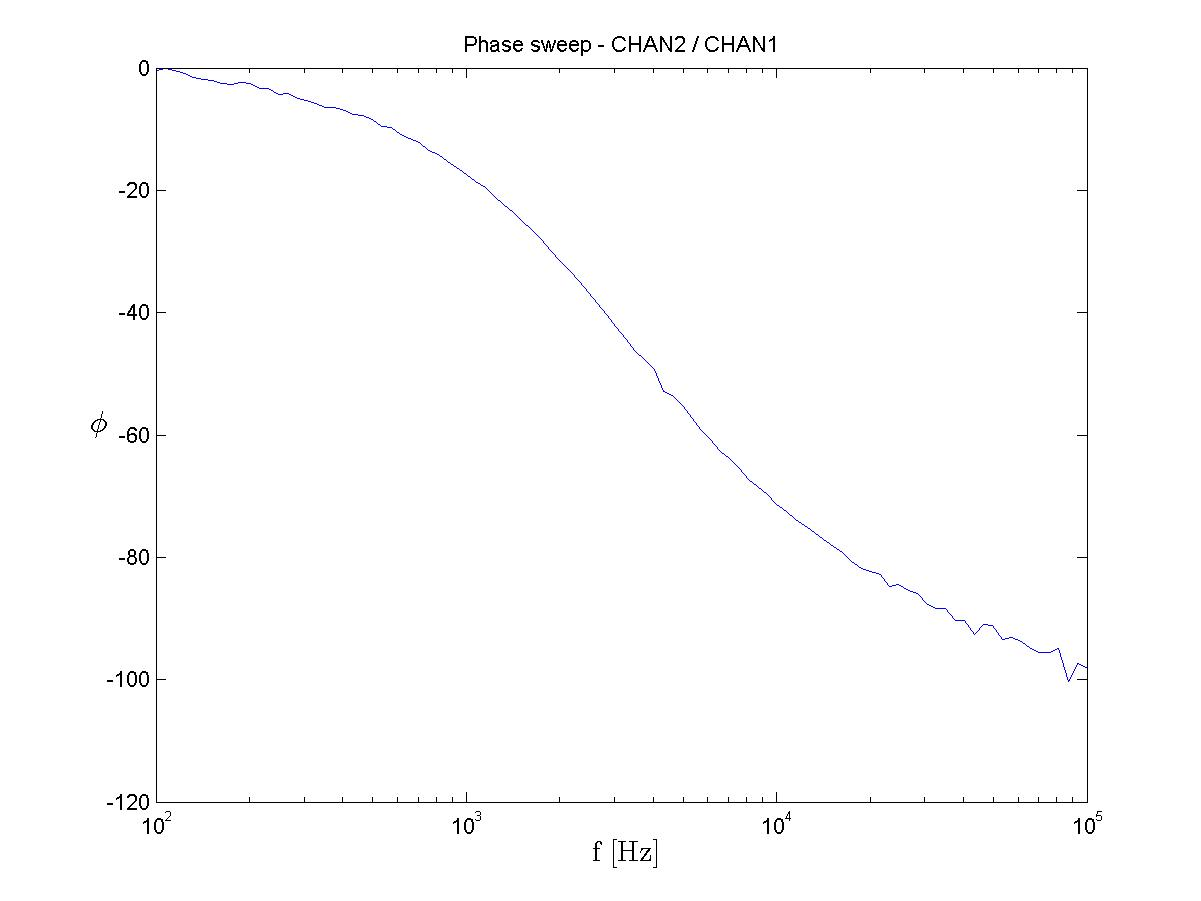
\includegraphics[width=0.9\textwidth]{1000OhmFreundlich_phasesweep_xlog.jpg}
                \caption{Bode-Diagramm mit $R_L = 1000\si{\ohm}$}
            \end{figure}
        \end{center}

        \textbf{Bemerkung:}

        Bei der Messung mit $R_L = 100\si{\ohm}$ wurde für das Phasendiagramm nur
        bis $f = 10^4\si{\hertz}$ geplottet, da das Signal $U_2$ an der Sekundärwicklung
        für große Frequenzen sehr stark rauschte, was dann zu Fehlern während des
        Freuency-sweeps führte. Auch die auffälligen Peaks bei kleinen Frequenzen
        sind mit großer Sicherheit Messfehler, da sie stark vom zuvor berechneten
        Plot abweichen. Der generelle Verlauf ist aber trotzdem klar zu erkennen.

\end{document}
